% \documentclass[11pt,twoside,a4paper]{article}
% \usepackage{times}

% \usepackage{xeCJK}

% \setmainfont{Times New Roman}

% \setCJKmainfont{Songti SC}
\documentclass[10pt]{ctexart}
% \usepackage[UTF-8]{ctex}
\usepackage{amsmath}
\usepackage{amsthm} % 根据 amsthm 的手册, amsthm 的加载要在 amsmath 之后
\usepackage{amssymb}  %为了能使用\mathbb{H} 
\usepackage{booktabs}
\usepackage{multirow}
\usepackage{tabularx}
\usepackage{xcolor}
\usepackage[colorlinks,linkcolor=blue]{hyperref} % 使用超链接
\usepackage{pdfpages}
\usepackage{geometry}
\geometry{a4paper,scale=0.8}
\usepackage{graphicx} %插入图片的宏包
\usepackage{float} %设置图片浮动位置的宏包
\usepackage{subfigure} %插入多图时用子图显示的宏包
\usepackage{graphicx}

\usepackage{listings}

\lstset{
 columns=fixed,       
 numbers=left,                                        % 在左侧显示行号
 numberstyle=\tiny\color{gray},                       % 设定行号格式
 frame=none,                                          % 不显示背景边框
 backgroundcolor=\color[RGB]{245,245,244},            % 设定背景颜色
 keywordstyle=\color[RGB]{40,40,255},                 % 设定关键字颜色
 numberstyle=\footnotesize\color{darkgray},           
 commentstyle=\it\color[RGB]{0,96,96},                % 设置代码注释的格式
 stringstyle=\rmfamily\slshape\color[RGB]{128,0,0},   % 设置字符串格式
 showstringspaces=false,                              % 不显示字符串中的空格
%language=c++,                                        % 设置语言
}

\newtheorem{definition}{定义}
\newtheorem{lemma}{引理}
\newtheorem{theorem}{定理}



\title{第 5 课 练习}
\author{谢文进}
\date{\today}
\begin{document}
\maketitle

\begin{enumerate}
    \item $KZG$ 多项式承诺方案在 $Setup$ 阶段涉及到计算对秘密评估点 $\tau$ 的幂的承诺,这被称为“可信设置”,通常在被称为“Powers of Tau”的仪式中利用多方计算生成。 假如说有一天,你在一张纸条上找到了 $\tau$ 的值。 你怎么能用它来制作一个假的 $KZG$ 证明呢?

    答:我们知道在Setup阶段的$\tau$值,原来的三个步骤:
    \begin{itemize}
        \item $Setup(1^\lambda,d) \rightarrow srs, srs =(ck,vk)=(\{[\tau^i]_1\}_{i=0}^{d-1},[\tau]_2)$.
        \item $Commit(ck;f(X)) \rightarrow C, f(X) = \sum_{i=0}^{n-1}f_iX^i, C = \sum_{i=0}^{n-1}[f_i][\tau^i]_1=[f(\tau)]_1$
        \item $Open(srs,C,x,y;f(X)) \rightarrow \{0,1\}$:
        \begin{enumerate}
            \item[a)] Prover 计算$q(X)=\frac{f(X)-y}{X-x}$, 发送证明$\pi = [q(\tau)]_1$;
            \item[b)] Verifier 验证$e(C-[y]_1, H) \overset{\text{?}}{=} e(\pi,[\tau]_2-[x]_2)$
        \end{enumerate}
    \end{itemize}
    如今,伪造者并不知道多项式$f(X)$,因此不能计算出$y$,对于一个伪造的$y'$(也就是$f(x) \neq y'$),想要通过发送证明$\pi_{Fake}$通过验证。现在伪造者想要验证者通过验证
    \begin{displaymath}
        \begin{aligned}
            e(\pi_{Fake},[\tau]_2-[x]_2) = e(C-[y']_1, H)\\
            \Rightarrow e(\pi_{Fake}, H)^{\tau - x} = e(C-[y']_1, H)\\
            \Rightarrow e(\pi_{Fake}, H) = e(C-[y']_1, H)^{\frac{1}{\tau - x}}\\
            \Rightarrow \pi_{Fake} = (C-[y']_1)^{\frac{1}{\tau - x}}
        \end{aligned}
    \end{displaymath}
    由此伪造出证明$\pi_{Fake}$.
    
    \item 从 $KZG$ 多项式承诺方案构造一个\textbf{向量承诺方案}。 (提示:对于向量 $m=\left(m_{1}, \ldots, m_{q}\right)$,是否存在一个“插值多项式”$I(X)$ 使得 $I\left(x_{i}\right)=y_{i}$?)
    \begin{center}
        \fcolorbox{black}{gray!10}{\parbox{.9\linewidth}{\textbf{有趣的事实}:Verkle 树\cite{VerkleTree}是一种使用向量承诺而不是哈希函数的 Merkle 树。 使用 KZG 向量承诺方案,您能看出为什么 Verkle 树更高效吗?}}
    \end{center}
    答:现在要对向量$m = (m_1,m_2,\cdots,m_q)$进行承诺,也就是允许证明任意位置$i$对应$m_i$。首先通过拉格朗日插值,使得一个多项式$f(X)$对任意$i$都有$f(i)=m_i$,根据插值公式,得到
    $$
    f(X) = \sum_{i=0}^{n-1}m_i \prod_{j=0, j\neq i}^{n-1}\frac{X-j}{i-j}.
    $$
    接着,KZG对该多项式$f(X)$进行承诺就可以了。

    如果证明一个元素,Merkle树需要$O(\log_2n)$大小来证明,而这里可以看到只需要$O(1)$就可以。论文\cite{VerkleTree}中给出了与Merkle树证明大小的比较:
    \begin{figure}[H]
        \centering
        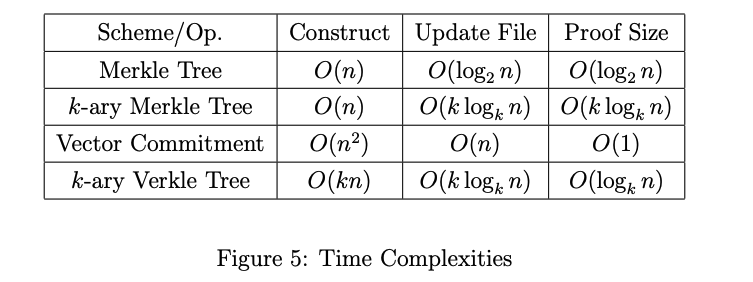
\includegraphics[width=0.7\textwidth]{img/VerkleTree.png} 
    \end{figure}

    \item $KZG$ 多项式承诺方案对关系 $p(x)=$ $y$ 进行披露证明 $\pi$。 你能扩展这个方案来产生一个多重证明 $\pi$,让我们相信 $p\left(x_{i}\right)=y_{i}$ 对于点列表和评估 $\left(x_{i }, y_{i}\right)$ ? (提示:假设您有一个插值多项式 $I(X)$ 使得 $I\left(x_{i}\right)=y_{i}$)。

    答:先构造一个拉格朗日插值多项式$I(X)$ 使得 $I\left(x_{i}\right)=y_{i}(i=0,\cdots, k-1)$,根据插值公式得
    $$
    I(X)=\sum_{i=0}^{k-1}y_i \prod_{j=0,j\neq i}^{k-1}\frac{X-x_j}{x_i-x_j}
    $$
    则$I(X)$的因子有$(X-x_1), \cdots, (X-x_{k-1})$,将它们相乘得到零多项式$g(X)=(X-x_1)\cdot (X-x_2) \cdots (X-x_{k-1})$。构造商多项式
    $$
    q(X)=\frac{p(X)-I(X)}{g(X)}
    $$
    由于$p(X)$也能整除$g(X)$,因此$q(X)$能整除$g(X)$.具体承诺方案如下:
    \begin{itemize}
        \item $Setup(1^\lambda,d) \rightarrow srs, srs =(ck,vk)=(\{[\tau^i]_1\}_{i=0}^{d-1},[\tau]_2)$.
        \item $Commit(ck;f(X)) \rightarrow C, p(X) = \sum_{i=0}^{n-1}p_iX^i, C = \sum_{i=0}^{n-1}[p_i][\tau^i]_1=[p(\tau)]_1$
        \item $Open(srs,C,(x_i,y_i);p(X)) \rightarrow \{0,1\}$:
            \begin{enumerate}
                \item[a)] Prover 根据$(x_i,y_i)$计算出$I(X)$与$g(X)$,接着计算$q(X)=\frac{p(X)-I(X)}{g(X)}$, 发送证明$\pi = [q(\tau)]_1$;
                \item[b)] Verifier 验证$e(C-[I(\tau)]_1, H) \overset{\text{?}}{=} e(\pi,[g(\tau)]_2)$.
            \end{enumerate}
    \end{itemize}
\end{enumerate}

\subsubsection*{英文原文}

1. The $Setup$ phase of the $KZG$ polynomial commitment scheme involves computing commitments to powers of a secret evaluation point $\tau$. This is called the "trusted setup" and is often generated in a multi-party computation known as the "Powers of Tau" ceremony. One day, you find the value of $\tau$ on a slip of paper. How can you use it to make a fake $KZG$ opening proof?

2. Construct a \textbf{vector commitment scheme} from the $KZG$ polynomial commitment scheme. (Hint: For a vector $m=\left(m_{1}, \ldots, m_{q}\right)$, is there an "interpolation polynomial" $I(X)$ such that $I(i)=m[i]$ ?)

\begin{center}
    \fcolorbox{black}{gray!10}{\parbox{.9\linewidth}{\textbf{Fun fact}:The Verkle tree \cite{VerkleTree} is a Merkle tree that uses a vector commitment instead of a hash function. Using the KZG vector commitment scheme, can you see why a Verkle tree is more efficient?}}
\end{center}

3. The $KZG$ polynomial commitment scheme makes an opening proof $\pi$ for the relation $p(x)=$ $y$. Can you extend the scheme to produce a multiproof $\pi$, that convinces us of $p\left(x_{i}\right)=y_{i}$ for a list of points and evaluations $\left(x_{i}, y_{i}\right)$ ? (Hint: assume that you have an interpolation polynomial $I(X)$ such that $I\left(x_{i}\right)=y_{i}$).

\begin{thebibliography}{10}
    \bibitem{VerkleTree}J. Kuszmaul, \href{https://math.mit.edu/research/highschool/primes/materials/2018/Kuszmaul.pdf}{https://math.mit.edu/research/highschool/primes/materials/2018/Kuszmaul.pdf}, 2019.  
    \bibitem{KZG}Dankrad Feist, \href{https://dankradfeist.de/ethereum/2020/06/16/kate-polynomial-commitments.html}{KZG多项式承诺}, 2020. 
\end{thebibliography}
\end{document}